% A short description of our team members
% I will add the outline of my description, just copy and paste it over and add your details -> also keep it aplhabetically -> see readMe for order of members

%start of member section
%WITHOUT STUFF THERE IS CHAOS :P 
\subsection{Elzahn Botha}
\begin{wrapfigure}[6]{l}{0.25\textwidth}
\vspace{10pt}
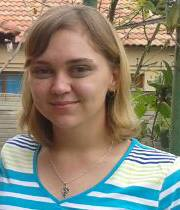
\includegraphics[width=80px]{ElzahnBotha.jpg}
\end{wrapfigure}

\textcolor{white}{.}
\subsubsection{Interests}
\begin{itemize}
	\item[-]{Video Games}
	\item[-]{Game development}
	\item[-]{Programming}
	\item[-]{Anime}
\end{itemize}
\subsubsection{Technical Skills} 
\begin{itemize}
	\item[-]{I have already been exposed to Java and been working with it for about a year now}
\end{itemize}
\subsubsection{Past Experience}
\begin{itemize}
	\item[-]{I have experience in writing programs and systems in Java}
\end{itemize}
\subsubsection{Non-Technical Strengths} 
\begin{itemize}
	\item[-]{Hard and dedicated worker}
	\item[-]{Always ready to learn new technologies and languages}
	\item[-]{Functions best under pressure}
\end{itemize}
\subsubsection{Why I want to do this project}
This project seemed like it would be a rather interesting project to do as well as the fact that it would be great exposure to a whole new side of IT that I have not yet had the privilege of delving into. I believe that by doing this project I will get valuable exposure that can later help in other projects that I might attempt. This project also seems like it would be a good challenge since I am more comfortable with smaller projects and systems and by doing a larger project such as this it will help me broaden my range of capabilities. Lastly due to the size of the project and the strict time line the pressure will be greatly increased helping me to work at my best without losing interest with the project. 

\subsection{Jason Richard Evans}
\begin{wrapfigure}[5]{l}{0.25\textwidth}
\vspace{10pt}

\includegraphics[width=80px]{Jason.jpg}
\end{wrapfigure}

\textcolor{white}{.}
\subsubsection{Interests} stuff 
\subsubsection{Technical Skills} stuff
\subsubsection{Past Experience} stuff 
\subsubsection{Non-Technical Strengths} stuff
\subsubsection{Why I want to do this project} stuff

\subsection{Renette Ros}
\begin{wrapfigure}[8]{l}{0.25\textwidth}
\vspace{10pt}
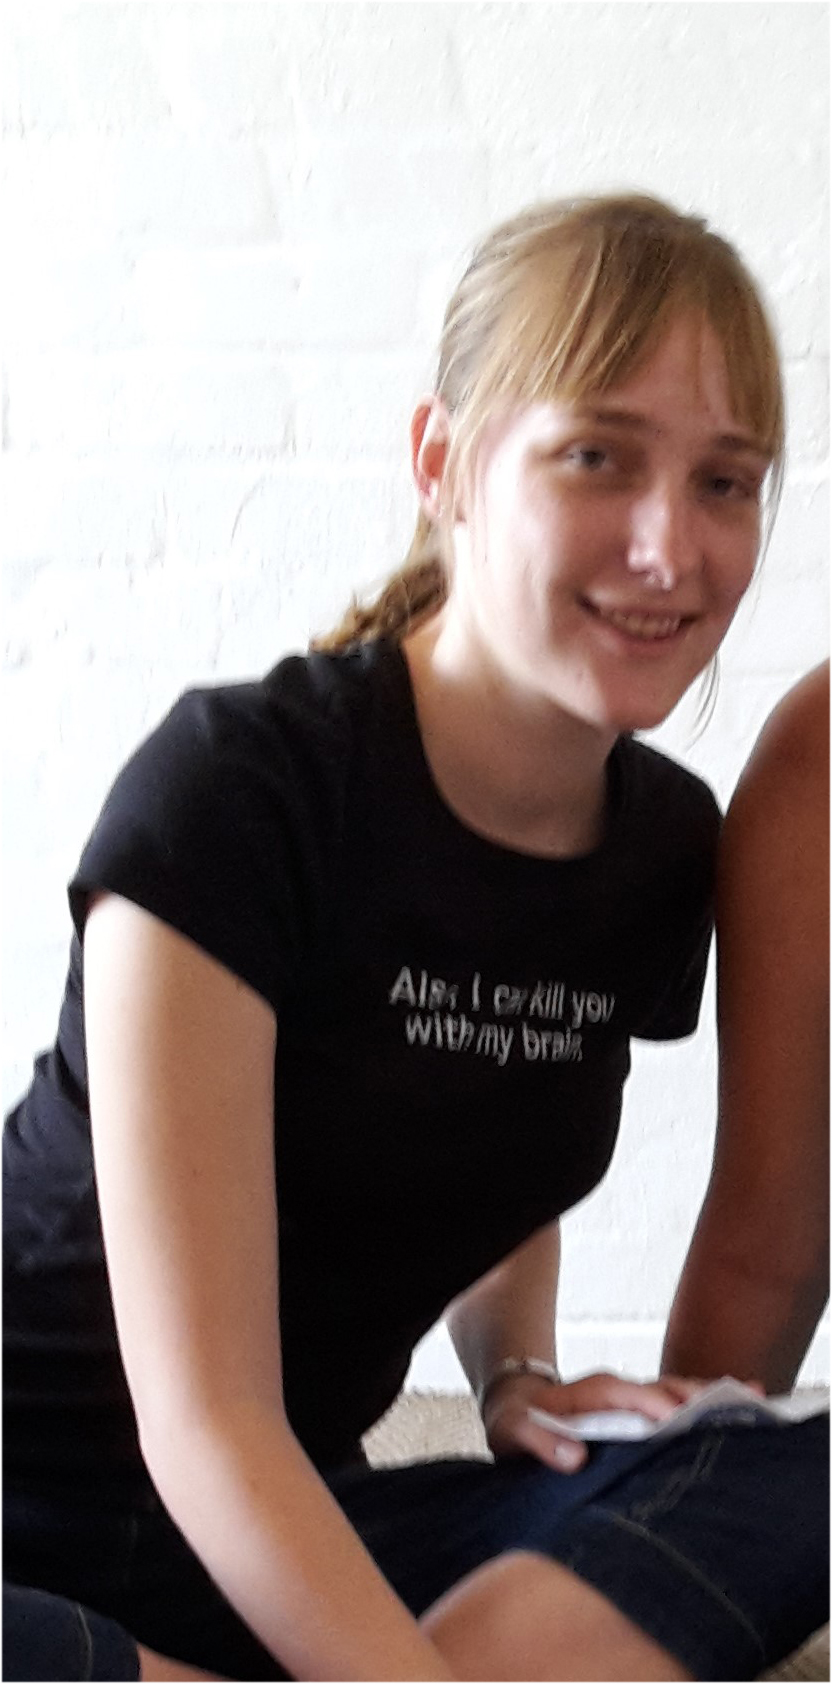
\includegraphics[width=80px]{Renette.jpg}
\vspace{10pt}
\end{wrapfigure}

\textcolor{white}{.}
\subsubsection{Interests} stuff
\subsubsection{Technical Skills} stuff
\subsubsection{Past Experience} stuff
\subsubsection{Non-Technical Strengths} stuff
\subsubsection{Why I want to do this project} stuff


\subsection{Szymon Ziolkowski}
\begin{wrapfigure}[5]{l}{0.25\textwidth}
\vspace{10pt}
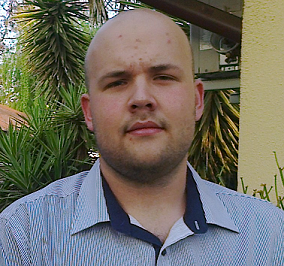
\includegraphics[width=80px]{Szymon.png}
\end{wrapfigure}

\textcolor{white}{.}
\subsubsection{Interests}
	\begin{itemize}
		\item Networks
		\item Security
		\item Computer hardware and electronics
		\item Paintball
		\item Video games
	\end{itemize}
\subsubsection{Technical Skills} 
	\begin{itemize}
		\item C\# and Java
		\item Web development
		\item SQLite, MySQL and SQL Server
	\end{itemize}
\subsubsection{Past Experience}
I have no past experience that might be relevant to the project. %dont forget to remove this%
\subsubsection{Non-Technical Strengths}
	\begin{itemize}
		\item Don't give up easily
		\item Helpful
	\end{itemize}
\subsubsection{Why I want to do this project} 


\subsection{Vivian Laura-Lee Venter}
\begin{wrapfigure}[7]{l}{0.25\textwidth}
\vspace{10pt}

\includegraphics[width=80px]{Vivian.png}
\end{wrapfigure}

\textcolor{white}{.}
\subsubsection{Interests} stuff
\subsubsection{Technical Skills} stuff
\subsubsection{Past Experience} stuff
\subsubsection{Non-Technical Strengths} stuff
\subsubsection{Why I want to do this project} stuff


\subsection{Tienie Pritchard}
\begin{wrapfigure}[7]{l}{0.25\textwidth}
\vspace{10pt}

\includegraphics[width=80px]{Tienie.jpg}
\end{wrapfigure}

\textcolor{white}{.}
\subsubsection{Interests} stuff
\subsubsection{Technical Skills} stuff
\subsubsection{Past Experience} stuff
\subsubsection{Non-Technical Strengths} stuff
\subsubsection{Why I want to do this project} stuff
%end of member section